% !TeX root = ../main.tex
\section{Kinetics Parameters}
\label{app:kinetics}

%\subsection{Summary of production routes}

% 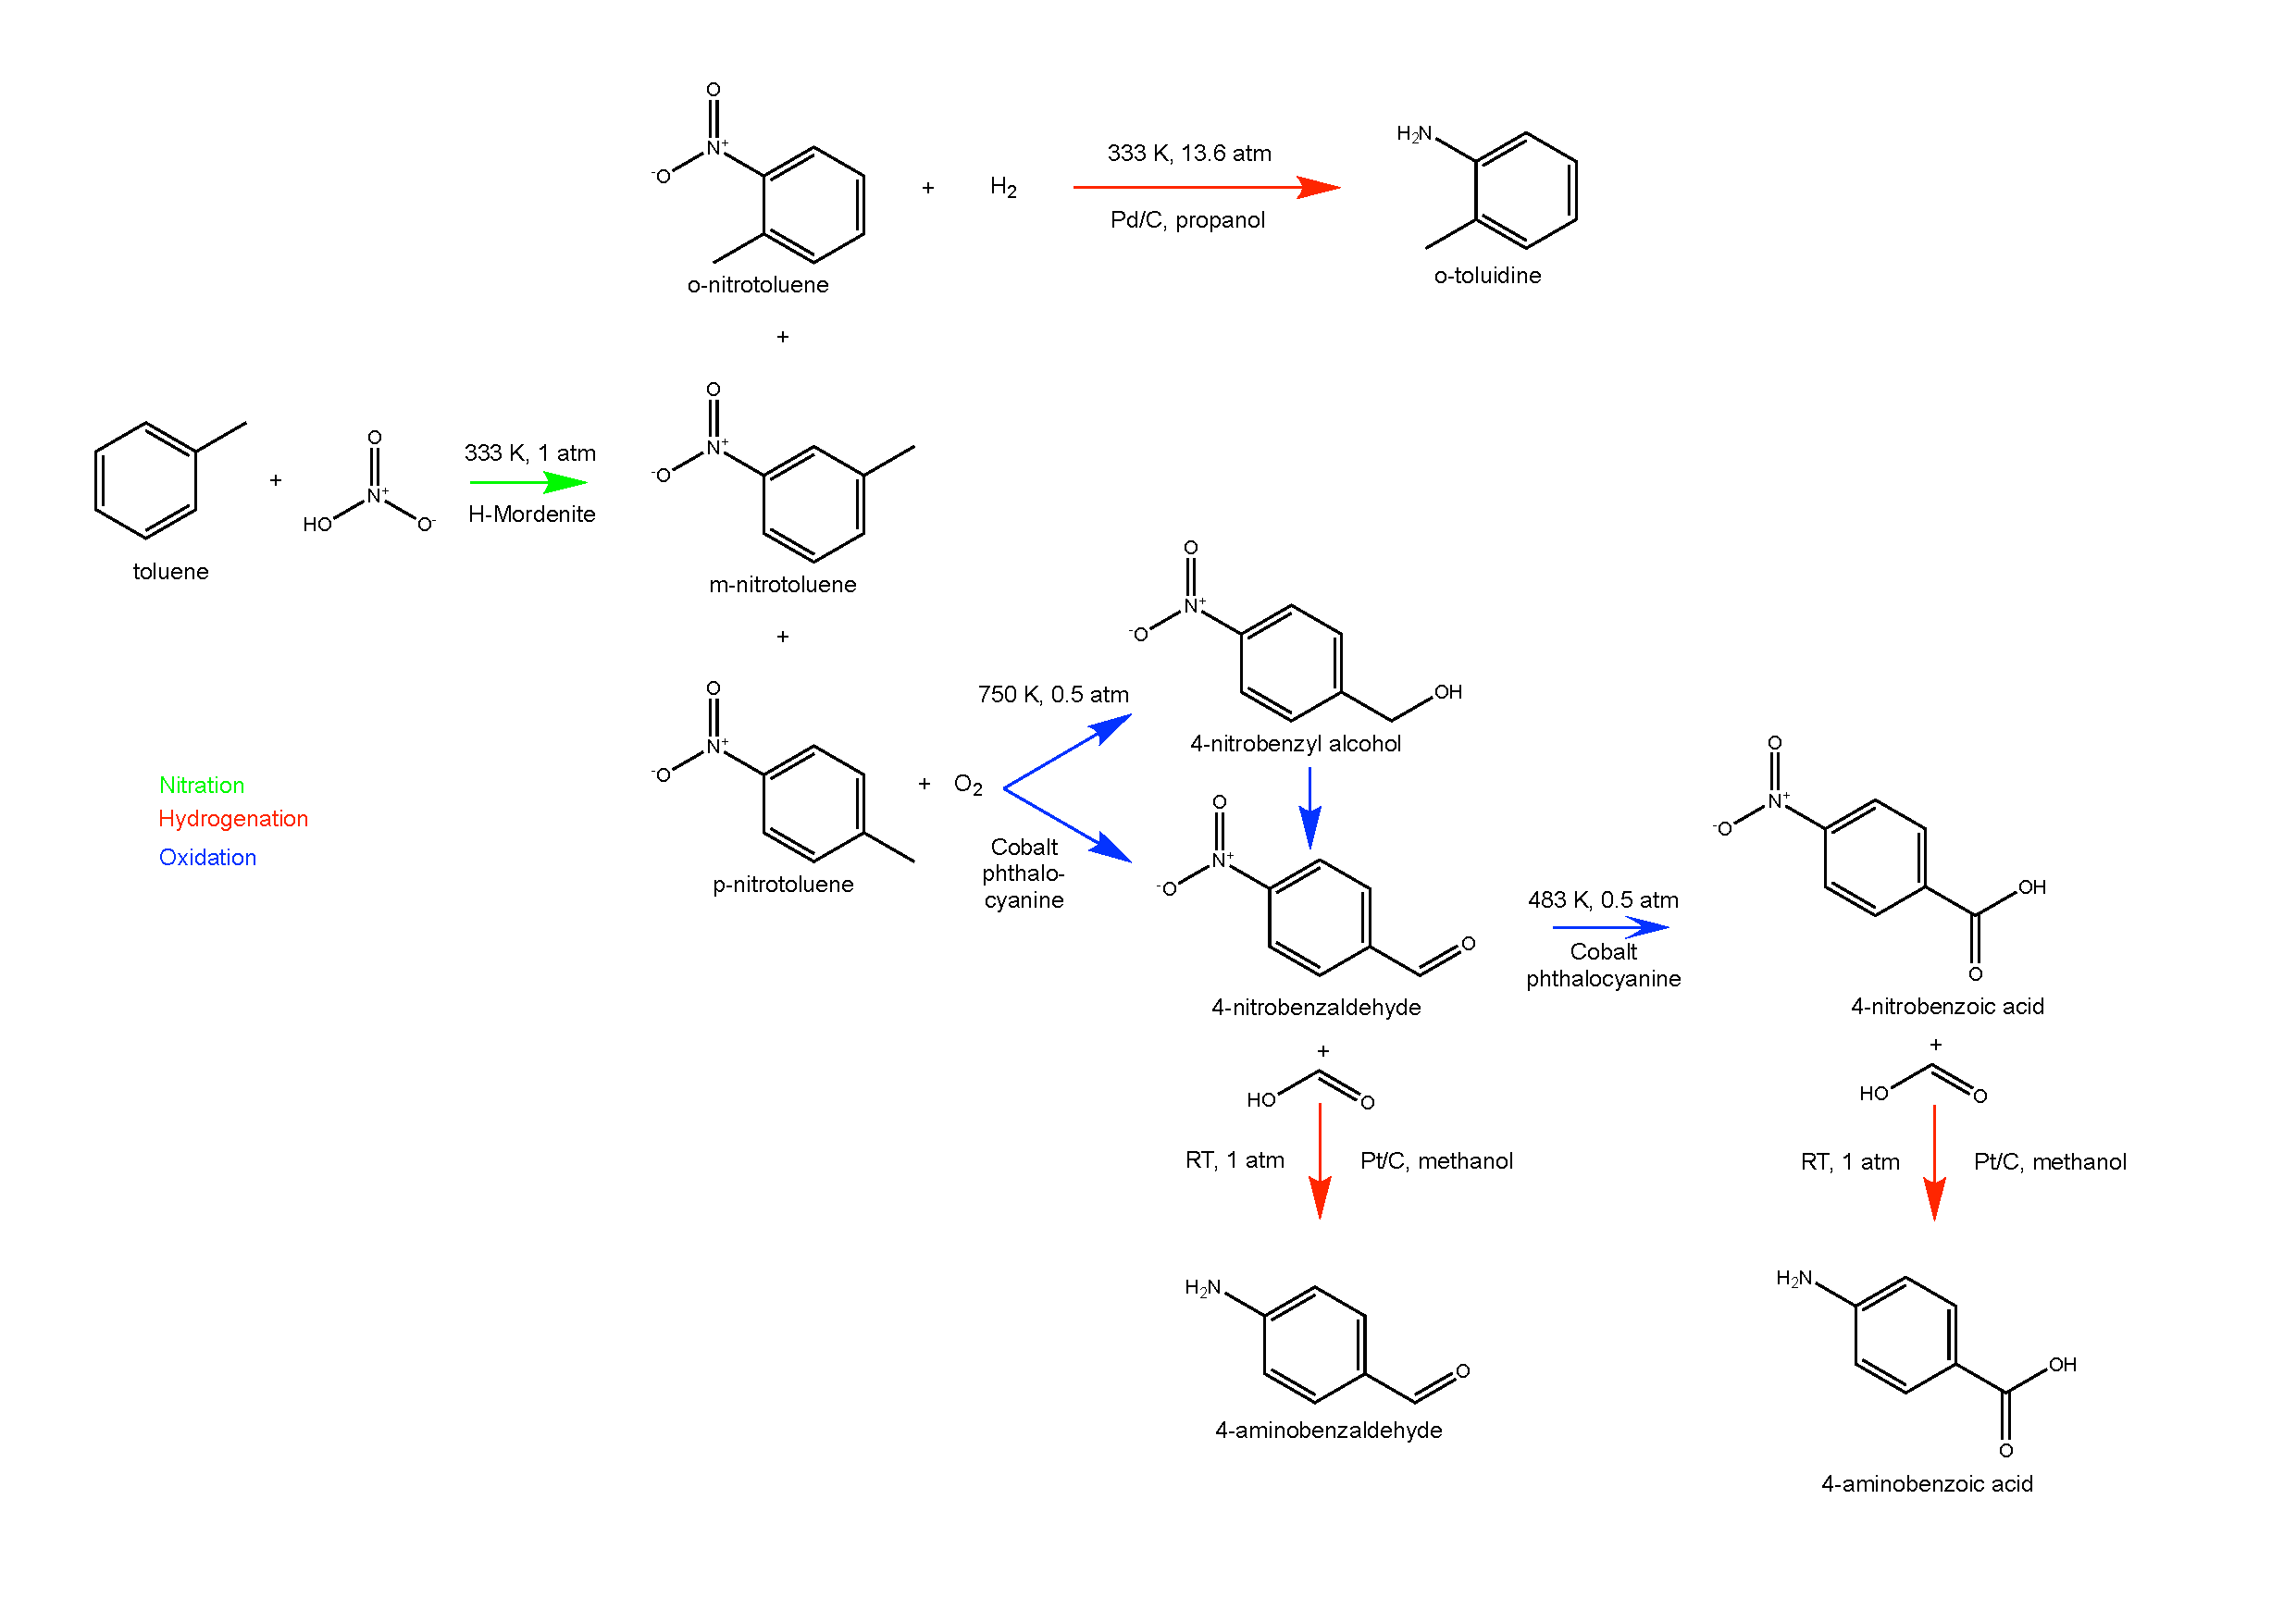
\includepdf[pages=-,landscape]{figures/routes-chosen.pdf}

\begin{landscape}
\begin{figure}[H]
    \centering
    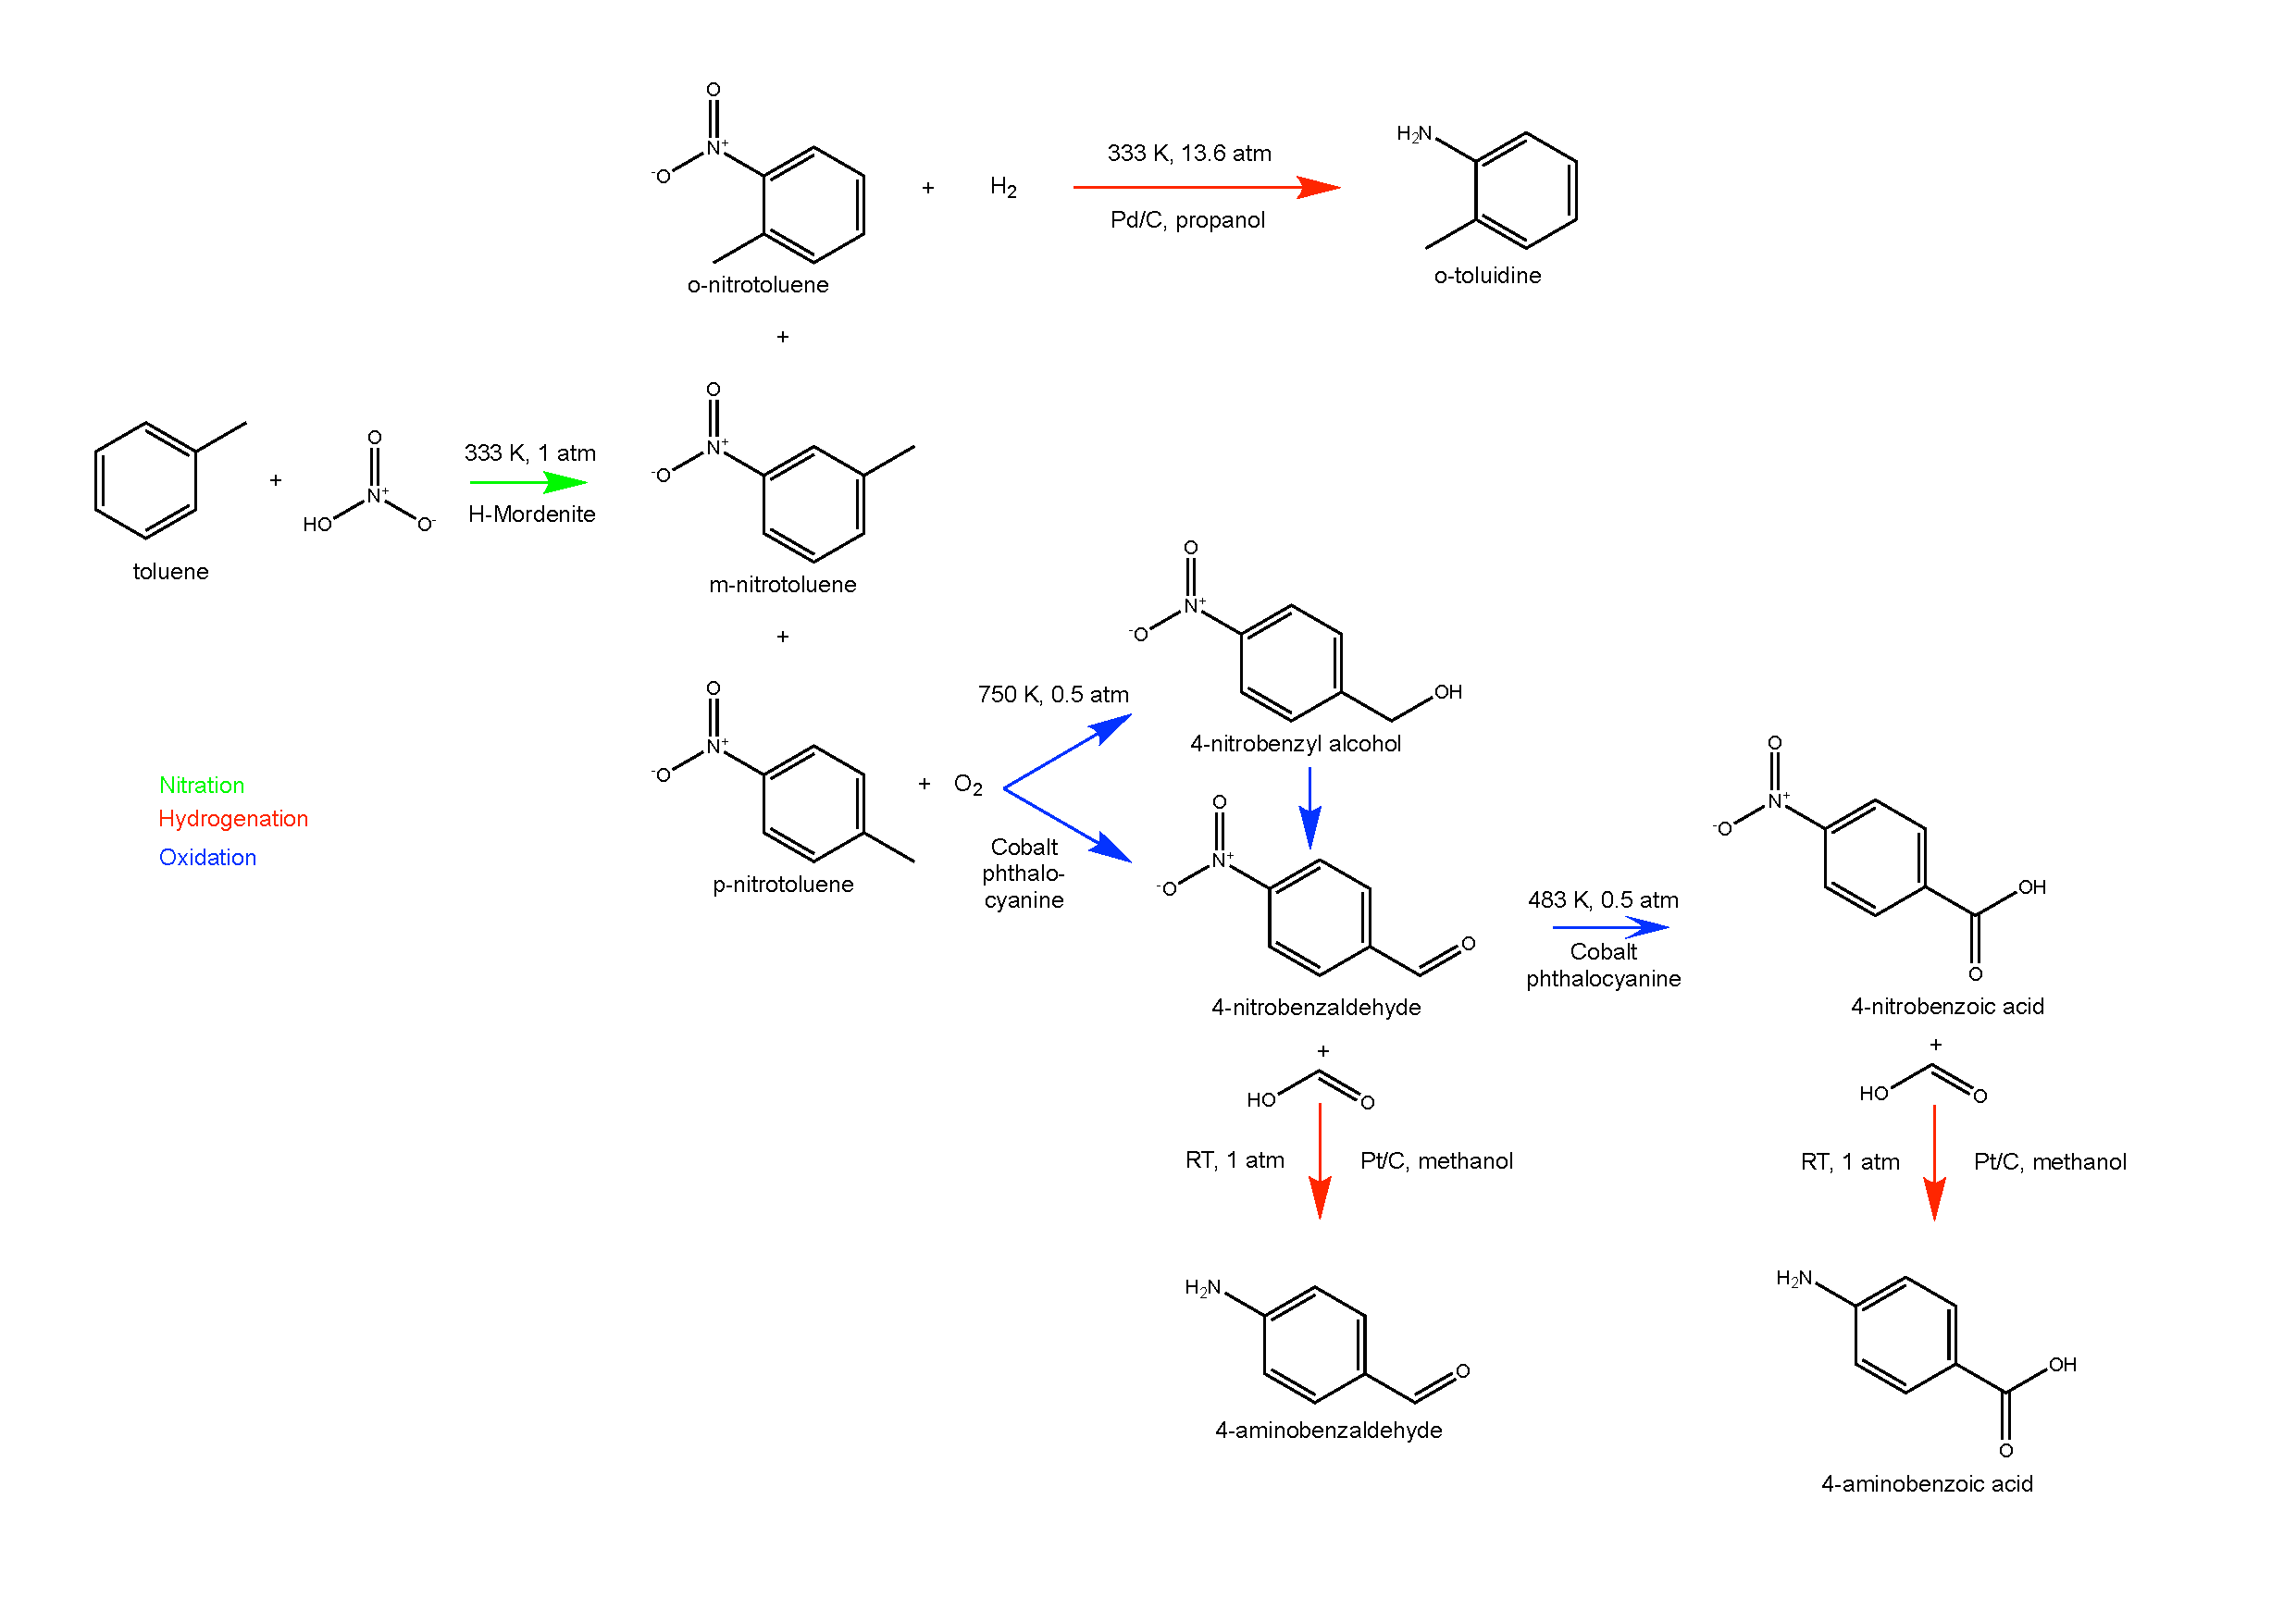
\includegraphics[width=0.8\linewidth]{figures/routes-chosen.pdf}
    \caption{Selected synthesis routes}
    \label{fig:routes-chosen}
\end{figure}
\end{landscape}


\subsection{Toluene nitration}
\paragraph{Assumptions}
\begin{itemize}
    \item The stoichiometric reaction is \ce{\mathrm{Toluene} +  \mathrm{Nitric}  \mathrm{acid} \rightarrow 0.44\mathrm{PNT} + 0.03 \mathrm{MNT} + 0.53 \mathrm{ONT} + \ch{H2O}}, where PNT, MTN and ONT are respectively the $para$, $ortho$ and $meta$ isomers of nitroltoluene.
    \item The ratio of isomers is reflected in the stoichiometric equt
    \item Negligible production of dinitrotoluene by-products as reported selectivity with H-Mordenite catalyst is lower than 0.55mol\% \cite{jeeru_kinetics_2018}.
    \item Kinetic parameters were obtained for a system free from mass transfer resistances and thus when the reaction is kinetically controlled \cite{jeeru_kinetics_2018}. Hence we can safely assume that the intrinsic rate of reaction was measures.
    \item The rate of reaction of toluene is first order in toluene and nitric acid concentrations. However with 2:1 mole ratio of nitric acid to toluene, the rate can be approximated to a pseudo-first order reaction with respect to toluene \cite{jeeru_kinetics_2018}.
    \begin{equation}
    \frac{dC_{toluene}}{dt}=k_1 \cdot C_{toluene} 
    \end{equation}
    \item The rate constant follows the Arrhenius law below:
    \begin{equation}
        
    \end{equation}
    \item The loss in activity of the catalyst was neglected \cite{jeeru_kinetics_2018}.
\end{itemize}





\subsection{o-nitrotoluene hydrogenation}

\subsection{4-nitrotoluene oxidation}

\subsection{Reduction of 4-nitrobenzaldehyde and 4-nitrobenzoic acid}